\documentclass[twoside]{book}

% Packages required by doxygen
\usepackage{fixltx2e}
\usepackage{calc}
\usepackage{doxygen}
\usepackage[export]{adjustbox} % also loads graphicx
\usepackage{graphicx}
\usepackage[utf8]{inputenc}
\usepackage{makeidx}
\usepackage{multicol}
\usepackage{multirow}
\PassOptionsToPackage{warn}{textcomp}
\usepackage{textcomp}
\usepackage[nointegrals]{wasysym}
\usepackage[table]{xcolor}

% Font selection
\usepackage[T1]{fontenc}
\usepackage[scaled=.90]{helvet}
\usepackage{courier}
\usepackage{amssymb}
\usepackage{sectsty}
\renewcommand{\familydefault}{\sfdefault}
\allsectionsfont{%
  \fontseries{bc}\selectfont%
  \color{darkgray}%
}
\renewcommand{\DoxyLabelFont}{%
  \fontseries{bc}\selectfont%
  \color{darkgray}%
}
\newcommand{\+}{\discretionary{\mbox{\scriptsize$\hookleftarrow$}}{}{}}

% Page & text layout
\usepackage{geometry}
\geometry{%
  a4paper,%
  top=2.5cm,%
  bottom=2.5cm,%
  left=2.5cm,%
  right=2.5cm%
}
\tolerance=750
\hfuzz=15pt
\hbadness=750
\setlength{\emergencystretch}{15pt}
\setlength{\parindent}{0cm}
\setlength{\parskip}{3ex plus 2ex minus 2ex}
\makeatletter
\renewcommand{\paragraph}{%
  \@startsection{paragraph}{4}{0ex}{-1.0ex}{1.0ex}{%
    \normalfont\normalsize\bfseries\SS@parafont%
  }%
}
\renewcommand{\subparagraph}{%
  \@startsection{subparagraph}{5}{0ex}{-1.0ex}{1.0ex}{%
    \normalfont\normalsize\bfseries\SS@subparafont%
  }%
}
\makeatother

% Headers & footers
\usepackage{fancyhdr}
\pagestyle{fancyplain}
\fancyhead[LE]{\fancyplain{}{\bfseries\thepage}}
\fancyhead[CE]{\fancyplain{}{}}
\fancyhead[RE]{\fancyplain{}{\bfseries\leftmark}}
\fancyhead[LO]{\fancyplain{}{\bfseries\rightmark}}
\fancyhead[CO]{\fancyplain{}{}}
\fancyhead[RO]{\fancyplain{}{\bfseries\thepage}}
\fancyfoot[LE]{\fancyplain{}{}}
\fancyfoot[CE]{\fancyplain{}{}}
\fancyfoot[RE]{\fancyplain{}{\bfseries\scriptsize Generated by Doxygen }}
\fancyfoot[LO]{\fancyplain{}{\bfseries\scriptsize Generated by Doxygen }}
\fancyfoot[CO]{\fancyplain{}{}}
\fancyfoot[RO]{\fancyplain{}{}}
\renewcommand{\footrulewidth}{0.4pt}
\renewcommand{\chaptermark}[1]{%
  \markboth{#1}{}%
}
\renewcommand{\sectionmark}[1]{%
  \markright{\thesection\ #1}%
}

% Indices & bibliography
\usepackage{natbib}
\usepackage[titles]{tocloft}
\setcounter{tocdepth}{3}
\setcounter{secnumdepth}{5}
\makeindex

% Hyperlinks (required, but should be loaded last)
\usepackage{ifpdf}
\ifpdf
  \usepackage[pdftex,pagebackref=true]{hyperref}
\else
  \usepackage[ps2pdf,pagebackref=true]{hyperref}
\fi
\hypersetup{%
  colorlinks=true,%
  linkcolor=blue,%
  citecolor=blue,%
  unicode%
}

% Custom commands
\newcommand{\clearemptydoublepage}{%
  \newpage{\pagestyle{empty}\cleardoublepage}%
}

\usepackage{caption}
\captionsetup{labelsep=space,justification=centering,font={bf},singlelinecheck=off,skip=4pt,position=top}

%===== C O N T E N T S =====

\begin{document}

% Titlepage & ToC
\hypersetup{pageanchor=false,
             bookmarksnumbered=true,
             pdfencoding=unicode
            }
\pagenumbering{alph}
\begin{titlepage}
\vspace*{7cm}
\begin{center}%
{\Large i\+Robot }\\
\vspace*{1cm}
{\large Generated by Doxygen 1.8.14}\\
\end{center}
\end{titlepage}
\clearemptydoublepage
\pagenumbering{roman}
\tableofcontents
\clearemptydoublepage
\pagenumbering{arabic}
\hypersetup{pageanchor=true}

%--- Begin generated contents ---
\chapter{Hierarchical Index}
\section{Class Hierarchy}
This inheritance list is sorted roughly, but not completely, alphabetically\+:\begin{DoxyCompactList}
\item Q\+Dialog\begin{DoxyCompactList}
\item \contentsline{section}{Order\+Window}{\pageref{class_order_window}}{}
\end{DoxyCompactList}
\item Q\+Widget\begin{DoxyCompactList}
\item \contentsline{section}{Product\+Window}{\pageref{class_product_window}}{}
\end{DoxyCompactList}
\end{DoxyCompactList}

\chapter{Class Index}
\section{Class List}
Here are the classes, structs, unions and interfaces with brief descriptions\+:\begin{DoxyCompactList}
\item\contentsline{section}{\mbox{\hyperlink{class_order_window}{Order\+Window}} }{\pageref{class_order_window}}{}
\item\contentsline{section}{\mbox{\hyperlink{class_product_window}{Product\+Window}} }{\pageref{class_product_window}}{}
\end{DoxyCompactList}

\chapter{Class Documentation}
\hypertarget{classadmin_screen}{}\section{admin\+Screen Class Reference}
\label{classadmin_screen}\index{admin\+Screen@{admin\+Screen}}


Inheritance diagram for admin\+Screen\+:\nopagebreak
\begin{figure}[H]
\begin{center}
\leavevmode
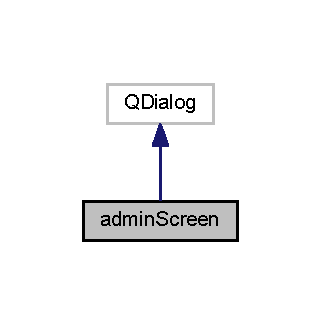
\includegraphics[width=154pt]{classadmin_screen__inherit__graph}
\end{center}
\end{figure}


Collaboration diagram for admin\+Screen\+:\nopagebreak
\begin{figure}[H]
\begin{center}
\leavevmode
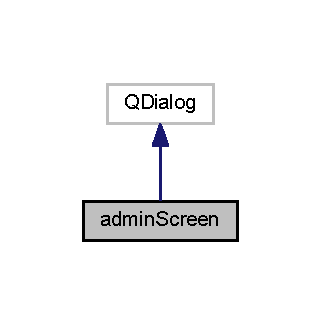
\includegraphics[width=154pt]{classadmin_screen__coll__graph}
\end{center}
\end{figure}
\subsection*{Public Member Functions}
\begin{DoxyCompactItemize}
\item 
\mbox{\Hypertarget{classadmin_screen_ae4f80dfbf6d56b9b0318cd44d95baf8c}\label{classadmin_screen_ae4f80dfbf6d56b9b0318cd44d95baf8c}} 
{\bfseries admin\+Screen} (Q\+Widget $\ast$parent=nullptr)
\end{DoxyCompactItemize}


The documentation for this class was generated from the following files\+:\begin{DoxyCompactItemize}
\item 
adminscreen.\+h\item 
adminscreen.\+cpp\end{DoxyCompactItemize}

\hypertarget{class_contact_us}{}\section{Contact\+Us Class Reference}
\label{class_contact_us}\index{Contact\+Us@{Contact\+Us}}


Inheritance diagram for Contact\+Us\+:\nopagebreak
\begin{figure}[H]
\begin{center}
\leavevmode
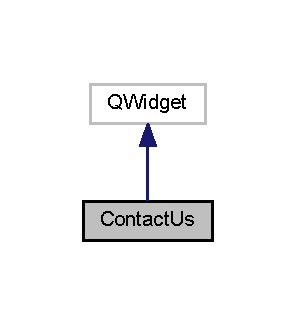
\includegraphics[width=142pt]{class_contact_us__inherit__graph}
\end{center}
\end{figure}


Collaboration diagram for Contact\+Us\+:\nopagebreak
\begin{figure}[H]
\begin{center}
\leavevmode
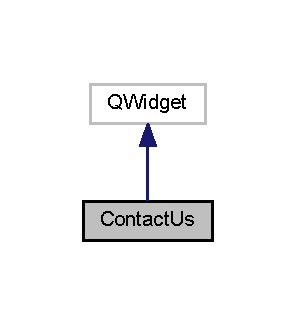
\includegraphics[width=142pt]{class_contact_us__coll__graph}
\end{center}
\end{figure}
\subsection*{Public Member Functions}
\begin{DoxyCompactItemize}
\item 
\mbox{\Hypertarget{class_contact_us_a6e20fc1c353d994a2f0bf13df4580232}\label{class_contact_us_a6e20fc1c353d994a2f0bf13df4580232}} 
{\bfseries Contact\+Us} (Q\+Widget $\ast$parent=nullptr)
\item 
\mbox{\Hypertarget{class_contact_us_a44bd80bbb4908c913bb07019a609c5ba}\label{class_contact_us_a44bd80bbb4908c913bb07019a609c5ba}} 
\mbox{\hyperlink{class_contact_us_a44bd80bbb4908c913bb07019a609c5ba}{$\sim$\+Contact\+Us}} ()
\begin{DoxyCompactList}\small\item\em Constructor. \end{DoxyCompactList}\end{DoxyCompactItemize}


The documentation for this class was generated from the following files\+:\begin{DoxyCompactItemize}
\item 
contactus.\+h\item 
contactus.\+cpp\end{DoxyCompactItemize}

\hypertarget{classcust_guarantee}{}\section{cust\+Guarantee Class Reference}
\label{classcust_guarantee}\index{cust\+Guarantee@{cust\+Guarantee}}


Inheritance diagram for cust\+Guarantee\+:\nopagebreak
\begin{figure}[H]
\begin{center}
\leavevmode
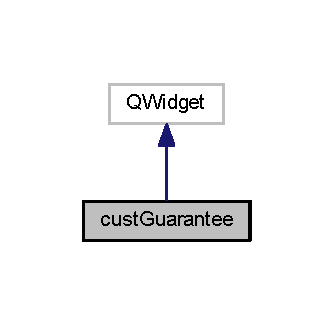
\includegraphics[width=160pt]{classcust_guarantee__inherit__graph}
\end{center}
\end{figure}


Collaboration diagram for cust\+Guarantee\+:\nopagebreak
\begin{figure}[H]
\begin{center}
\leavevmode
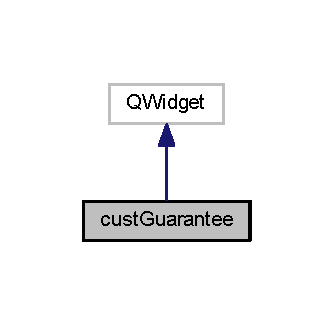
\includegraphics[width=160pt]{classcust_guarantee__coll__graph}
\end{center}
\end{figure}
\subsection*{Public Member Functions}
\begin{DoxyCompactItemize}
\item 
\mbox{\Hypertarget{classcust_guarantee_ad4a1fbde7c9422147f6b0a15e1abe930}\label{classcust_guarantee_ad4a1fbde7c9422147f6b0a15e1abe930}} 
\mbox{\hyperlink{classcust_guarantee_ad4a1fbde7c9422147f6b0a15e1abe930}{cust\+Guarantee}} (Q\+Widget $\ast$parent=nullptr)
\begin{DoxyCompactList}\small\item\em Constructor. \end{DoxyCompactList}\item 
\mbox{\Hypertarget{classcust_guarantee_a2fb1d22a1052a21ae5ff15589dad2c27}\label{classcust_guarantee_a2fb1d22a1052a21ae5ff15589dad2c27}} 
\mbox{\hyperlink{classcust_guarantee_a2fb1d22a1052a21ae5ff15589dad2c27}{$\sim$cust\+Guarantee}} ()
\begin{DoxyCompactList}\small\item\em Destructor. \end{DoxyCompactList}\end{DoxyCompactItemize}


The documentation for this class was generated from the following files\+:\begin{DoxyCompactItemize}
\item 
custguarantee.\+h\item 
custguarantee.\+cpp\end{DoxyCompactItemize}

\hypertarget{classcustomer}{}\section{customer Class Reference}
\label{classcustomer}\index{customer@{customer}}
\subsection*{Public Member Functions}
\begin{DoxyCompactItemize}
\item 
\mbox{\Hypertarget{classcustomer_a5634bb18127a7deddfea0323afffd275}\label{classcustomer_a5634bb18127a7deddfea0323afffd275}} 
{\bfseries customer} (Q\+String company, Q\+String address, Q\+String key, Q\+String interest)
\item 
\mbox{\Hypertarget{classcustomer_ace8662bdc59605411ff94c7bd119f15a}\label{classcustomer_ace8662bdc59605411ff94c7bd119f15a}} 
{\bfseries customer} (const \mbox{\hyperlink{classcustomer}{customer}} \&old)
\item 
\mbox{\Hypertarget{classcustomer_a42b1873e8a37d03cefd5f709055cf106}\label{classcustomer_a42b1873e8a37d03cefd5f709055cf106}} 
Q\+String {\bfseries get\+Company} ()
\item 
\mbox{\Hypertarget{classcustomer_adcdecf730cce4ec72d0f0e7fa6366bf5}\label{classcustomer_adcdecf730cce4ec72d0f0e7fa6366bf5}} 
Q\+String {\bfseries get\+Address} ()
\item 
\mbox{\Hypertarget{classcustomer_a51755d598e47029f9d496851be58a2a4}\label{classcustomer_a51755d598e47029f9d496851be58a2a4}} 
Q\+String {\bfseries get\+Key} ()
\item 
\mbox{\Hypertarget{classcustomer_abb319d9aed162ca748db58717a548ee3}\label{classcustomer_abb319d9aed162ca748db58717a548ee3}} 
Q\+String {\bfseries get\+Interest} ()
\end{DoxyCompactItemize}


The documentation for this class was generated from the following files\+:\begin{DoxyCompactItemize}
\item 
customer.\+h\item 
customer.\+cpp\end{DoxyCompactItemize}

\hypertarget{class_customer_screen}{}\section{Customer\+Screen Class Reference}
\label{class_customer_screen}\index{Customer\+Screen@{Customer\+Screen}}


Inheritance diagram for Customer\+Screen\+:\nopagebreak
\begin{figure}[H]
\begin{center}
\leavevmode
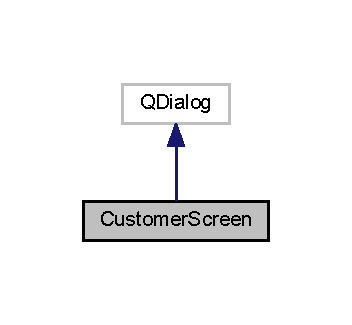
\includegraphics[width=169pt]{class_customer_screen__inherit__graph}
\end{center}
\end{figure}


Collaboration diagram for Customer\+Screen\+:\nopagebreak
\begin{figure}[H]
\begin{center}
\leavevmode
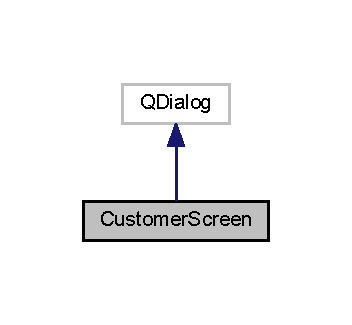
\includegraphics[width=169pt]{class_customer_screen__coll__graph}
\end{center}
\end{figure}
\subsection*{Public Member Functions}
\begin{DoxyCompactItemize}
\item 
\mbox{\Hypertarget{class_customer_screen_a85504dee21d3b41ba89c5084ac0d66d0}\label{class_customer_screen_a85504dee21d3b41ba89c5084ac0d66d0}} 
{\bfseries Customer\+Screen} (Q\+Widget $\ast$parent=nullptr)
\end{DoxyCompactItemize}


The documentation for this class was generated from the following files\+:\begin{DoxyCompactItemize}
\item 
customerscreen.\+h\item 
customerscreen.\+cpp\end{DoxyCompactItemize}

\hypertarget{class_main_window}{}\section{Main\+Window Class Reference}
\label{class_main_window}\index{Main\+Window@{Main\+Window}}


Inheritance diagram for Main\+Window\+:\nopagebreak
\begin{figure}[H]
\begin{center}
\leavevmode
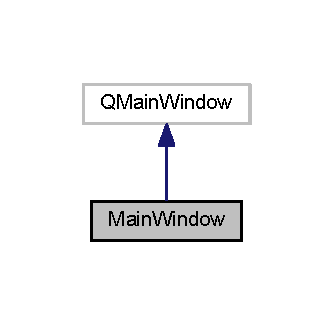
\includegraphics[width=160pt]{class_main_window__inherit__graph}
\end{center}
\end{figure}


Collaboration diagram for Main\+Window\+:\nopagebreak
\begin{figure}[H]
\begin{center}
\leavevmode
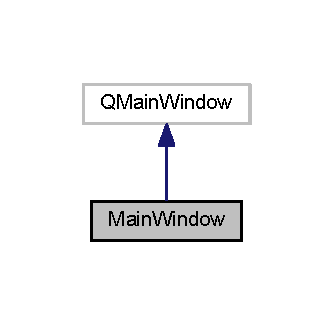
\includegraphics[width=160pt]{class_main_window__coll__graph}
\end{center}
\end{figure}
\subsection*{Public Slots}
\begin{DoxyCompactItemize}
\item 
\mbox{\Hypertarget{class_main_window_a91d73d4813d9994c8959a85997861960}\label{class_main_window_a91d73d4813d9994c8959a85997861960}} 
void {\bfseries admin\+Login} ()
\item 
\mbox{\Hypertarget{class_main_window_a9cce5254834fcf5848fd4afb1abcc4b0}\label{class_main_window_a9cce5254834fcf5848fd4afb1abcc4b0}} 
void {\bfseries customer\+Login} ()
\item 
\mbox{\Hypertarget{class_main_window_ab2539ea587be5e2abde872300d475df7}\label{class_main_window_ab2539ea587be5e2abde872300d475df7}} 
void {\bfseries logout} ()
\item 
void \mbox{\hyperlink{class_main_window_aa76b76e15140b8d87926542b0cbee9a3}{view\+Products}} ()
\begin{DoxyCompactList}\small\item\em Customer Window button to view Products Window. \end{DoxyCompactList}\item 
\mbox{\Hypertarget{class_main_window_a14784497acafa7c9b035f036466d8225}\label{class_main_window_a14784497acafa7c9b035f036466d8225}} 
void {\bfseries contacts} ()
\item 
\mbox{\Hypertarget{class_main_window_ac48e37766a3bbee22cb82fd32ed6b30b}\label{class_main_window_ac48e37766a3bbee22cb82fd32ed6b30b}} 
void {\bfseries view\+Guarantee} ()
\item 
\mbox{\Hypertarget{class_main_window_a185c3927a39f35758683d821fe16d3a7}\label{class_main_window_a185c3927a39f35758683d821fe16d3a7}} 
void {\bfseries help} ()
\item 
\mbox{\Hypertarget{class_main_window_a660d1b4fd70db9d4fffb6621098ddcc4}\label{class_main_window_a660d1b4fd70db9d4fffb6621098ddcc4}} 
void {\bfseries request\+Pamphlet} ()
\item 
\mbox{\Hypertarget{class_main_window_aaab61053a622840f65c394771133b28a}\label{class_main_window_aaab61053a622840f65c394771133b28a}} 
void {\bfseries view\+Customer\+List} ()
\item 
\mbox{\Hypertarget{class_main_window_a92b8246bb9207990c0cc41a2a9390bdd}\label{class_main_window_a92b8246bb9207990c0cc41a2a9390bdd}} 
void {\bfseries populate} ()
\item 
\mbox{\Hypertarget{class_main_window_a661e495fc5b587dce8c7b930120098aa}\label{class_main_window_a661e495fc5b587dce8c7b930120098aa}} 
void {\bfseries add\+Customer} ()
\item 
\mbox{\Hypertarget{class_main_window_afff9ca5b1b867af6b54eb1c8d9501522}\label{class_main_window_afff9ca5b1b867af6b54eb1c8d9501522}} 
void {\bfseries edit\+Customer} ()
\item 
\mbox{\Hypertarget{class_main_window_a95365ee88b53639217f8463916a15da4}\label{class_main_window_a95365ee88b53639217f8463916a15da4}} 
void {\bfseries delete\+Customer} ()
\item 
\mbox{\Hypertarget{class_main_window_a2a5b8c23beabae0461b4356ad2a0b14f}\label{class_main_window_a2a5b8c23beabae0461b4356ad2a0b14f}} 
void {\bfseries view\+Reviews} ()
\item 
\mbox{\Hypertarget{class_main_window_af9b5f9919c32f23211364ac62f55df91}\label{class_main_window_af9b5f9919c32f23211364ac62f55df91}} 
void {\bfseries key} ()
\item 
\mbox{\Hypertarget{class_main_window_af87f2e8818e039003c7f8e0d69ba8544}\label{class_main_window_af87f2e8818e039003c7f8e0d69ba8544}} 
void {\bfseries break\+Everything} ()
\item 
void \mbox{\hyperlink{class_main_window_ab27be7a4e38509990a9e2bbb0d77f26c}{on\+\_\+\+R\+P\+Main\+Request\+Pamphlet\+Button\+\_\+clicked}} ()
\begin{DoxyCompactList}\small\item\em Customer Window button to view Request Pamphlet Form. \end{DoxyCompactList}\item 
void \mbox{\hyperlink{class_main_window_ad8dc42f06d44432f03794e52d3970d19}{on\+\_\+\+R\+P\+Submit\+Button\+\_\+clicked}} ()
\begin{DoxyCompactList}\small\item\em Request Pamphlet Form submit button action. \end{DoxyCompactList}\end{DoxyCompactItemize}
\subsection*{Public Member Functions}
\begin{DoxyCompactItemize}
\item 
\mbox{\Hypertarget{class_main_window_a996c5a2b6f77944776856f08ec30858d}\label{class_main_window_a996c5a2b6f77944776856f08ec30858d}} 
{\bfseries Main\+Window} (Q\+Widget $\ast$parent=nullptr)
\item 
\mbox{\Hypertarget{class_main_window_a6dff16b4a5343ec7d147afbb566c2638}\label{class_main_window_a6dff16b4a5343ec7d147afbb566c2638}} 
\mbox{\hyperlink{classcustomer}{customer}} $\ast$ {\bfseries get\+Customer} ()
\end{DoxyCompactItemize}


\subsection{Member Function Documentation}
\mbox{\Hypertarget{class_main_window_ab27be7a4e38509990a9e2bbb0d77f26c}\label{class_main_window_ab27be7a4e38509990a9e2bbb0d77f26c}} 
\index{Main\+Window@{Main\+Window}!on\+\_\+\+R\+P\+Main\+Request\+Pamphlet\+Button\+\_\+clicked@{on\+\_\+\+R\+P\+Main\+Request\+Pamphlet\+Button\+\_\+clicked}}
\index{on\+\_\+\+R\+P\+Main\+Request\+Pamphlet\+Button\+\_\+clicked@{on\+\_\+\+R\+P\+Main\+Request\+Pamphlet\+Button\+\_\+clicked}!Main\+Window@{Main\+Window}}
\subsubsection{\texorpdfstring{on\+\_\+\+R\+P\+Main\+Request\+Pamphlet\+Button\+\_\+clicked}{on\_RPMainRequestPamphletButton\_clicked}}
{\footnotesize\ttfamily void Main\+Window\+::on\+\_\+\+R\+P\+Main\+Request\+Pamphlet\+Button\+\_\+clicked (\begin{DoxyParamCaption}{ }\end{DoxyParamCaption})\hspace{0.3cm}{\ttfamily [slot]}}



Customer Window button to view Request Pamphlet Form. 

Opens the Request Pamplet Form Window \mbox{\Hypertarget{class_main_window_ad8dc42f06d44432f03794e52d3970d19}\label{class_main_window_ad8dc42f06d44432f03794e52d3970d19}} 
\index{Main\+Window@{Main\+Window}!on\+\_\+\+R\+P\+Submit\+Button\+\_\+clicked@{on\+\_\+\+R\+P\+Submit\+Button\+\_\+clicked}}
\index{on\+\_\+\+R\+P\+Submit\+Button\+\_\+clicked@{on\+\_\+\+R\+P\+Submit\+Button\+\_\+clicked}!Main\+Window@{Main\+Window}}
\subsubsection{\texorpdfstring{on\+\_\+\+R\+P\+Submit\+Button\+\_\+clicked}{on\_RPSubmitButton\_clicked}}
{\footnotesize\ttfamily void Main\+Window\+::on\+\_\+\+R\+P\+Submit\+Button\+\_\+clicked (\begin{DoxyParamCaption}{ }\end{DoxyParamCaption})\hspace{0.3cm}{\ttfamily [slot]}}



Request Pamphlet Form submit button action. 

Saves request pamphlet inputs to variable members \mbox{\Hypertarget{class_main_window_aa76b76e15140b8d87926542b0cbee9a3}\label{class_main_window_aa76b76e15140b8d87926542b0cbee9a3}} 
\index{Main\+Window@{Main\+Window}!view\+Products@{view\+Products}}
\index{view\+Products@{view\+Products}!Main\+Window@{Main\+Window}}
\subsubsection{\texorpdfstring{view\+Products}{viewProducts}}
{\footnotesize\ttfamily void Main\+Window\+::view\+Products (\begin{DoxyParamCaption}{ }\end{DoxyParamCaption})\hspace{0.3cm}{\ttfamily [slot]}}



Customer Window button to view Products Window. 

Opens the Products Window (popup) 

The documentation for this class was generated from the following files\+:\begin{DoxyCompactItemize}
\item 
mainwindow.\+h\item 
mainwindow.\+cpp\end{DoxyCompactItemize}

\hypertarget{class_order_window}{}\section{Order\+Window Class Reference}
\label{class_order_window}\index{Order\+Window@{Order\+Window}}


Inheritance diagram for Order\+Window\+:\nopagebreak
\begin{figure}[H]
\begin{center}
\leavevmode
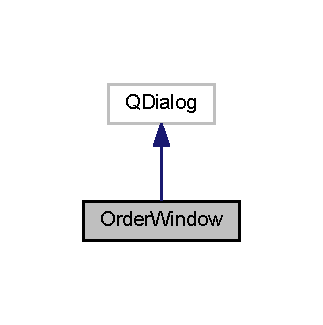
\includegraphics[width=155pt]{class_order_window__inherit__graph}
\end{center}
\end{figure}


Collaboration diagram for Order\+Window\+:\nopagebreak
\begin{figure}[H]
\begin{center}
\leavevmode
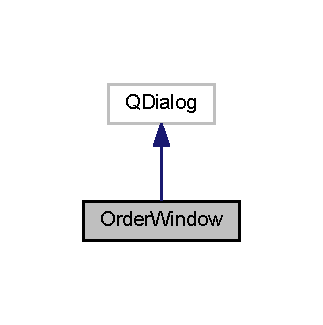
\includegraphics[width=155pt]{class_order_window__coll__graph}
\end{center}
\end{figure}
\subsection*{Public Member Functions}
\begin{DoxyCompactItemize}
\item 
\mbox{\Hypertarget{class_order_window_a4e93bee57fd21c5454cb0729ff43ace8}\label{class_order_window_a4e93bee57fd21c5454cb0729ff43ace8}} 
\mbox{\hyperlink{class_order_window_a4e93bee57fd21c5454cb0729ff43ace8}{Order\+Window}} (Q\+Widget $\ast$parent=nullptr)
\begin{DoxyCompactList}\small\item\em Constructor. \end{DoxyCompactList}\item 
\mbox{\Hypertarget{class_order_window_a127e3637720468474c85a9c4a1e150ac}\label{class_order_window_a127e3637720468474c85a9c4a1e150ac}} 
\mbox{\hyperlink{class_order_window_a127e3637720468474c85a9c4a1e150ac}{$\sim$\+Order\+Window}} ()
\begin{DoxyCompactList}\small\item\em Destructor. \end{DoxyCompactList}\item 
void \mbox{\hyperlink{class_order_window_a4fec739fb9e3c2c06fdf8afa7d94a4f9}{set\+Robot\+A\+Subtotal}} ()
\begin{DoxyCompactList}\small\item\em Sets and displays the subtotal for Robot A. \end{DoxyCompactList}\item 
void \mbox{\hyperlink{class_order_window_aa575a53f391f6bc103e89f2bf2fce91e}{set\+Robot\+B\+Subtotal}} ()
\begin{DoxyCompactList}\small\item\em Sets and displays the subtotal for Robot B. \end{DoxyCompactList}\item 
void \mbox{\hyperlink{class_order_window_a5283f60b1a3076038b08160b37542fdc}{set\+Robot\+C\+Subtotal}} ()
\begin{DoxyCompactList}\small\item\em Sets and displays the subtotal for Robot C. \end{DoxyCompactList}\item 
void \mbox{\hyperlink{class_order_window_a9b1e24f50bfc70c3920932f58331f917}{set\+Order\+Subtotal}} ()
\begin{DoxyCompactList}\small\item\em Sets and displays updated subtotal. \end{DoxyCompactList}\item 
void \mbox{\hyperlink{class_order_window_aa2a0cfb3003fd66954cc540dd9db23b8}{set\+Order\+Shipping}} ()
\begin{DoxyCompactList}\small\item\em Sets the order shipping \& handling charge displayed or hidden. \end{DoxyCompactList}\item 
void \mbox{\hyperlink{class_order_window_a6dfbb77a1a8911cc789062c6c00b7fe5}{set\+Order\+Sales\+Tax}} ()
\begin{DoxyCompactList}\small\item\em Sets and displays updated sales tax amount. \end{DoxyCompactList}\item 
void \mbox{\hyperlink{class_order_window_af1b6d198cf89a68c63afa28bc986786a}{set\+Order\+Total\+Price}} ()
\begin{DoxyCompactList}\small\item\em Sets and displays updated total price for order. \end{DoxyCompactList}\end{DoxyCompactItemize}


\subsection{Member Function Documentation}
\mbox{\Hypertarget{class_order_window_a6dfbb77a1a8911cc789062c6c00b7fe5}\label{class_order_window_a6dfbb77a1a8911cc789062c6c00b7fe5}} 
\index{Order\+Window@{Order\+Window}!set\+Order\+Sales\+Tax@{set\+Order\+Sales\+Tax}}
\index{set\+Order\+Sales\+Tax@{set\+Order\+Sales\+Tax}!Order\+Window@{Order\+Window}}
\subsubsection{\texorpdfstring{set\+Order\+Sales\+Tax()}{setOrderSalesTax()}}
{\footnotesize\ttfamily void Order\+Window\+::set\+Order\+Sales\+Tax (\begin{DoxyParamCaption}{ }\end{DoxyParamCaption})}



Sets and displays updated sales tax amount. 

sales\+Tax = ((subtotal + S\+H\+I\+P\+P\+I\+NG)$\ast$\+T\+A\+X\+\_\+\+R\+A\+TE); Here is the caller graph for this function\+:\nopagebreak
\begin{figure}[H]
\begin{center}
\leavevmode
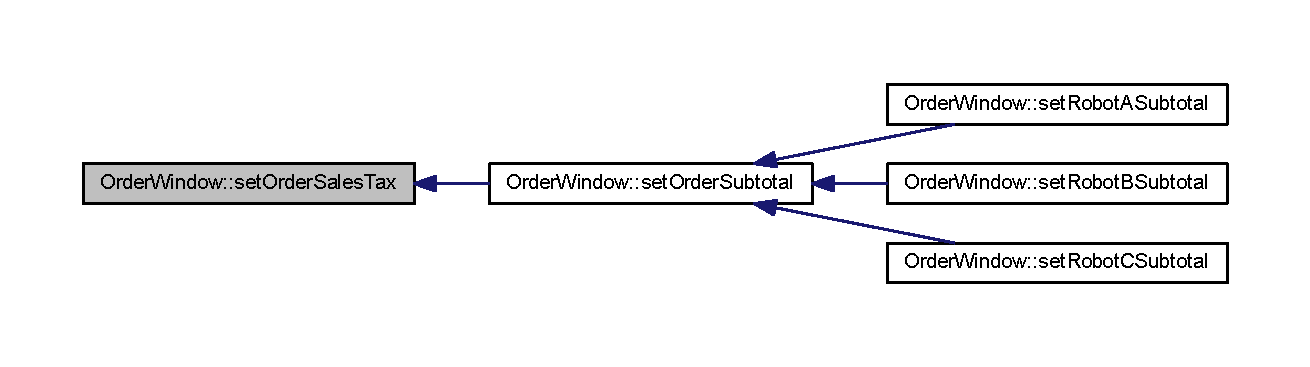
\includegraphics[width=350pt]{class_order_window_a6dfbb77a1a8911cc789062c6c00b7fe5_icgraph}
\end{center}
\end{figure}
\mbox{\Hypertarget{class_order_window_aa2a0cfb3003fd66954cc540dd9db23b8}\label{class_order_window_aa2a0cfb3003fd66954cc540dd9db23b8}} 
\index{Order\+Window@{Order\+Window}!set\+Order\+Shipping@{set\+Order\+Shipping}}
\index{set\+Order\+Shipping@{set\+Order\+Shipping}!Order\+Window@{Order\+Window}}
\subsubsection{\texorpdfstring{set\+Order\+Shipping()}{setOrderShipping()}}
{\footnotesize\ttfamily void Order\+Window\+::set\+Order\+Shipping (\begin{DoxyParamCaption}{ }\end{DoxyParamCaption})}



Sets the order shipping \& handling charge displayed or hidden. 

If subtotal $>$ 0, display shipping \& handling flat rate charge else, hide shipping \& handling flat rate charge Here is the caller graph for this function\+:\nopagebreak
\begin{figure}[H]
\begin{center}
\leavevmode
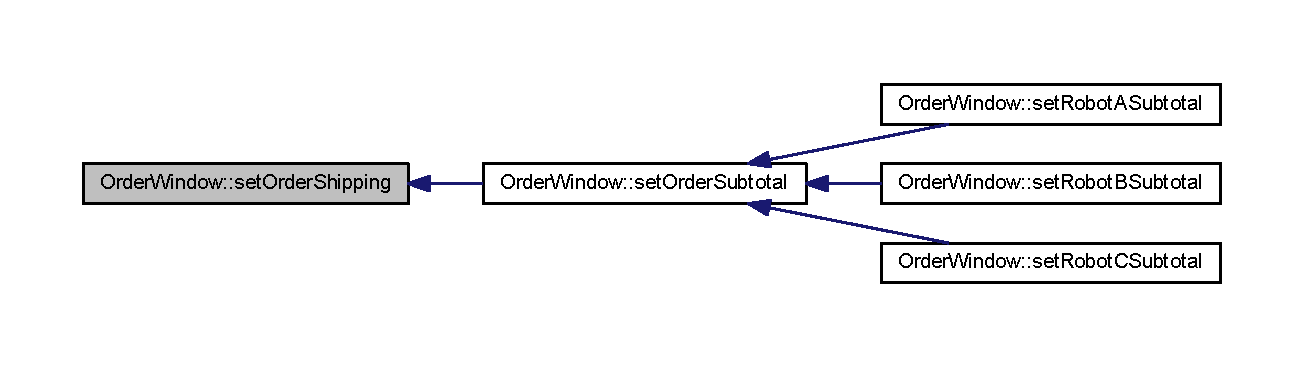
\includegraphics[width=350pt]{class_order_window_aa2a0cfb3003fd66954cc540dd9db23b8_icgraph}
\end{center}
\end{figure}
\mbox{\Hypertarget{class_order_window_a9b1e24f50bfc70c3920932f58331f917}\label{class_order_window_a9b1e24f50bfc70c3920932f58331f917}} 
\index{Order\+Window@{Order\+Window}!set\+Order\+Subtotal@{set\+Order\+Subtotal}}
\index{set\+Order\+Subtotal@{set\+Order\+Subtotal}!Order\+Window@{Order\+Window}}
\subsubsection{\texorpdfstring{set\+Order\+Subtotal()}{setOrderSubtotal()}}
{\footnotesize\ttfamily void Order\+Window\+::set\+Order\+Subtotal (\begin{DoxyParamCaption}{ }\end{DoxyParamCaption})}



Sets and displays updated subtotal. 

subtotal = robot\+A\+Subtotal + robot\+B\+Subtotal + robot\+C\+Subtotal; Here is the call graph for this function\+:\nopagebreak
\begin{figure}[H]
\begin{center}
\leavevmode
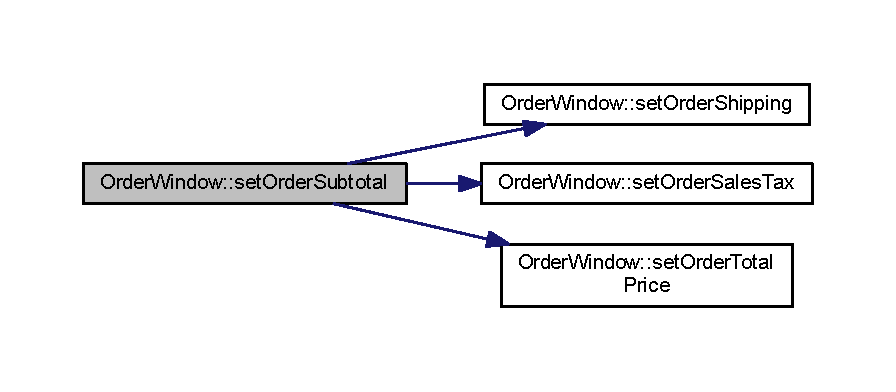
\includegraphics[width=350pt]{class_order_window_a9b1e24f50bfc70c3920932f58331f917_cgraph}
\end{center}
\end{figure}
Here is the caller graph for this function\+:\nopagebreak
\begin{figure}[H]
\begin{center}
\leavevmode
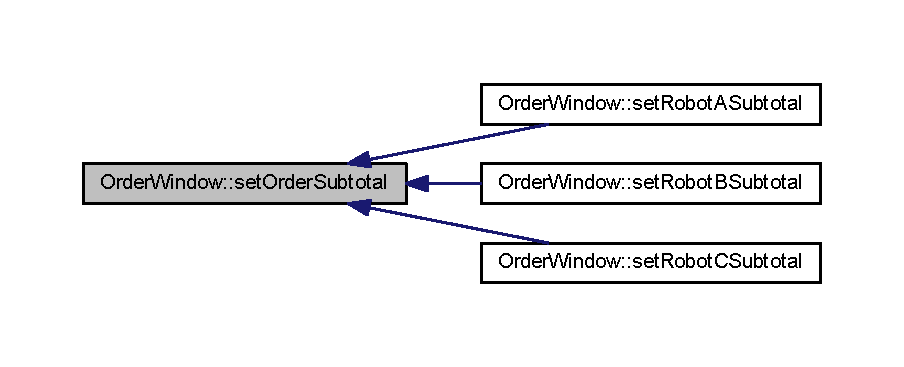
\includegraphics[width=350pt]{class_order_window_a9b1e24f50bfc70c3920932f58331f917_icgraph}
\end{center}
\end{figure}
\mbox{\Hypertarget{class_order_window_af1b6d198cf89a68c63afa28bc986786a}\label{class_order_window_af1b6d198cf89a68c63afa28bc986786a}} 
\index{Order\+Window@{Order\+Window}!set\+Order\+Total\+Price@{set\+Order\+Total\+Price}}
\index{set\+Order\+Total\+Price@{set\+Order\+Total\+Price}!Order\+Window@{Order\+Window}}
\subsubsection{\texorpdfstring{set\+Order\+Total\+Price()}{setOrderTotalPrice()}}
{\footnotesize\ttfamily void Order\+Window\+::set\+Order\+Total\+Price (\begin{DoxyParamCaption}{ }\end{DoxyParamCaption})}



Sets and displays updated total price for order. 

total\+Price = subtotal + S\+H\+I\+P\+P\+I\+NG + sales\+Tax; Here is the caller graph for this function\+:\nopagebreak
\begin{figure}[H]
\begin{center}
\leavevmode
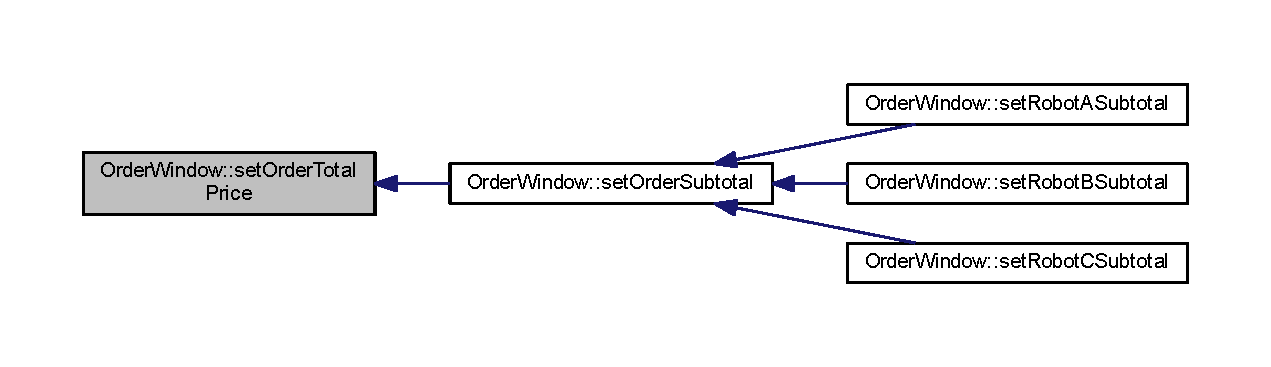
\includegraphics[width=350pt]{class_order_window_af1b6d198cf89a68c63afa28bc986786a_icgraph}
\end{center}
\end{figure}
\mbox{\Hypertarget{class_order_window_a4fec739fb9e3c2c06fdf8afa7d94a4f9}\label{class_order_window_a4fec739fb9e3c2c06fdf8afa7d94a4f9}} 
\index{Order\+Window@{Order\+Window}!set\+Robot\+A\+Subtotal@{set\+Robot\+A\+Subtotal}}
\index{set\+Robot\+A\+Subtotal@{set\+Robot\+A\+Subtotal}!Order\+Window@{Order\+Window}}
\subsubsection{\texorpdfstring{set\+Robot\+A\+Subtotal()}{setRobotASubtotal()}}
{\footnotesize\ttfamily void Order\+Window\+::set\+Robot\+A\+Subtotal (\begin{DoxyParamCaption}{ }\end{DoxyParamCaption})}



Sets and displays the subtotal for Robot A. 

robot\+A\+Subtotal = robot\+A\+Qty $\ast$ (R\+O\+B\+O\+T\+\_\+\+A\+\_\+\+P\+R\+I\+CE + (plan price)); Purchase button enabled if any robot qty $>$ 0 Here is the call graph for this function\+:\nopagebreak
\begin{figure}[H]
\begin{center}
\leavevmode
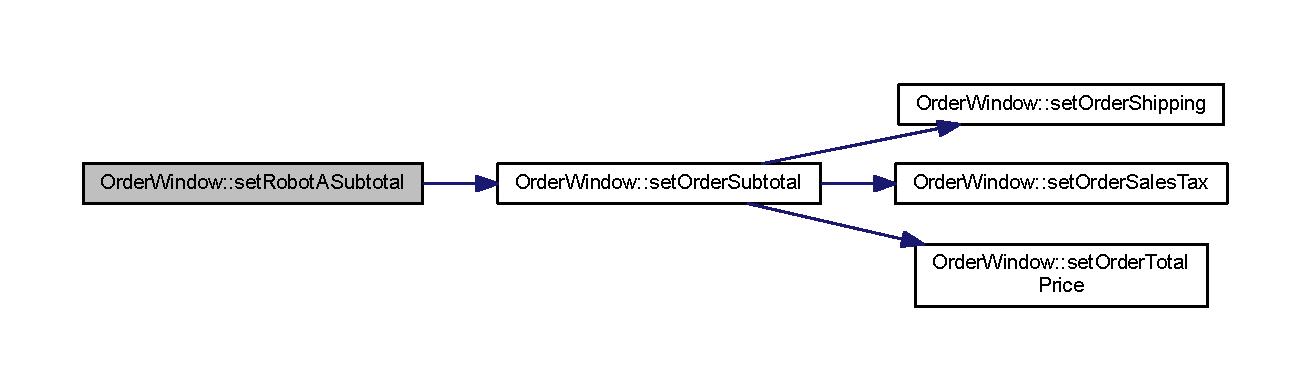
\includegraphics[width=350pt]{class_order_window_a4fec739fb9e3c2c06fdf8afa7d94a4f9_cgraph}
\end{center}
\end{figure}
\mbox{\Hypertarget{class_order_window_aa575a53f391f6bc103e89f2bf2fce91e}\label{class_order_window_aa575a53f391f6bc103e89f2bf2fce91e}} 
\index{Order\+Window@{Order\+Window}!set\+Robot\+B\+Subtotal@{set\+Robot\+B\+Subtotal}}
\index{set\+Robot\+B\+Subtotal@{set\+Robot\+B\+Subtotal}!Order\+Window@{Order\+Window}}
\subsubsection{\texorpdfstring{set\+Robot\+B\+Subtotal()}{setRobotBSubtotal()}}
{\footnotesize\ttfamily void Order\+Window\+::set\+Robot\+B\+Subtotal (\begin{DoxyParamCaption}{ }\end{DoxyParamCaption})}



Sets and displays the subtotal for Robot B. 

robot\+B\+Subtotal = robot\+B\+Qty $\ast$ (R\+O\+B\+O\+T\+\_\+\+B\+\_\+\+P\+R\+I\+CE + (plan price)); Purchase button enabled if any robot qty $>$ 0 Here is the call graph for this function\+:\nopagebreak
\begin{figure}[H]
\begin{center}
\leavevmode
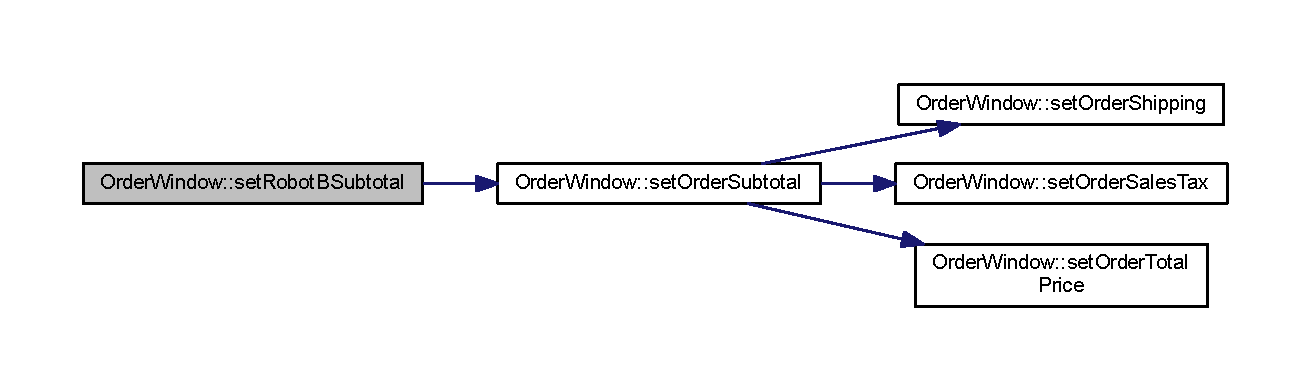
\includegraphics[width=350pt]{class_order_window_aa575a53f391f6bc103e89f2bf2fce91e_cgraph}
\end{center}
\end{figure}
\mbox{\Hypertarget{class_order_window_a5283f60b1a3076038b08160b37542fdc}\label{class_order_window_a5283f60b1a3076038b08160b37542fdc}} 
\index{Order\+Window@{Order\+Window}!set\+Robot\+C\+Subtotal@{set\+Robot\+C\+Subtotal}}
\index{set\+Robot\+C\+Subtotal@{set\+Robot\+C\+Subtotal}!Order\+Window@{Order\+Window}}
\subsubsection{\texorpdfstring{set\+Robot\+C\+Subtotal()}{setRobotCSubtotal()}}
{\footnotesize\ttfamily void Order\+Window\+::set\+Robot\+C\+Subtotal (\begin{DoxyParamCaption}{ }\end{DoxyParamCaption})}



Sets and displays the subtotal for Robot C. 

robot\+C\+Subtotal = robot\+C\+Qty $\ast$ (R\+O\+B\+O\+T\+\_\+\+C\+\_\+\+P\+R\+I\+CE + (plan price)); Purchase button enabled if any robot qty $>$ 0 Here is the call graph for this function\+:\nopagebreak
\begin{figure}[H]
\begin{center}
\leavevmode
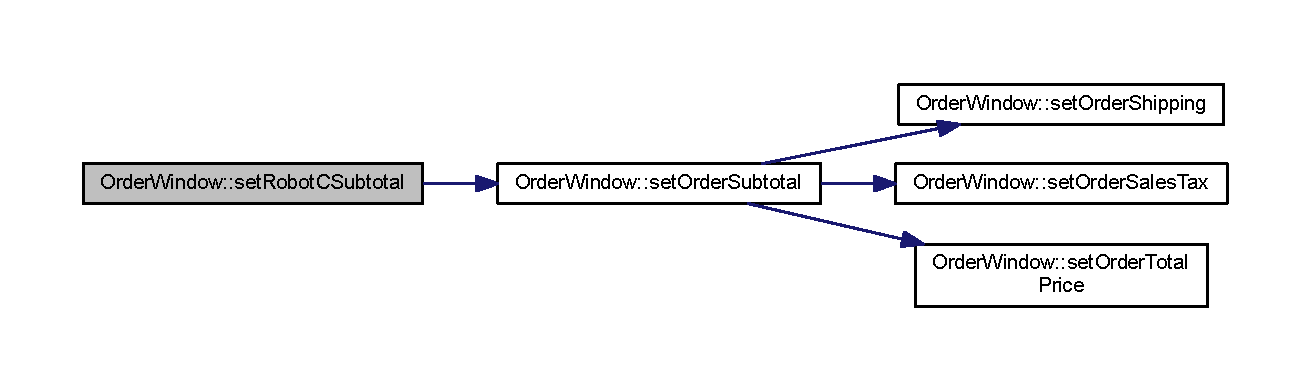
\includegraphics[width=350pt]{class_order_window_a5283f60b1a3076038b08160b37542fdc_cgraph}
\end{center}
\end{figure}


The documentation for this class was generated from the following files\+:\begin{DoxyCompactItemize}
\item 
order\+Window.\+h\item 
order\+Window.\+cpp\end{DoxyCompactItemize}

\hypertarget{class_product_window}{}\section{Product\+Window Class Reference}
\label{class_product_window}\index{Product\+Window@{Product\+Window}}


Inheritance diagram for Product\+Window\+:\nopagebreak
\begin{figure}[H]
\begin{center}
\leavevmode
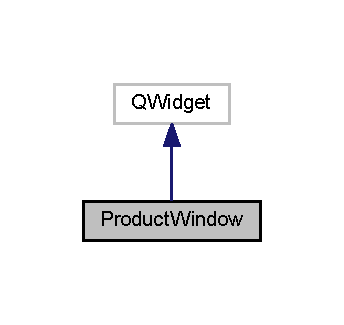
\includegraphics[width=165pt]{class_product_window__inherit__graph}
\end{center}
\end{figure}


Collaboration diagram for Product\+Window\+:\nopagebreak
\begin{figure}[H]
\begin{center}
\leavevmode
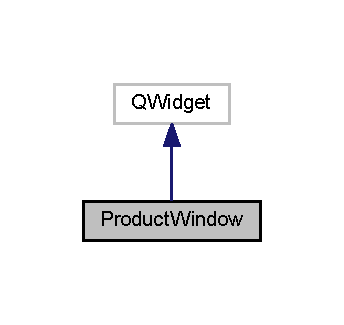
\includegraphics[width=165pt]{class_product_window__coll__graph}
\end{center}
\end{figure}
\subsection*{Public Member Functions}
\begin{DoxyCompactItemize}
\item 
\mbox{\Hypertarget{class_product_window_adafa731eb2e3c47c30f7a740a3a12576}\label{class_product_window_adafa731eb2e3c47c30f7a740a3a12576}} 
\mbox{\hyperlink{class_product_window_adafa731eb2e3c47c30f7a740a3a12576}{Product\+Window}} (Q\+Widget $\ast$parent=nullptr)
\begin{DoxyCompactList}\small\item\em Constructor. \end{DoxyCompactList}\item 
\mbox{\Hypertarget{class_product_window_ae113591d990345573cbcf9faf790a7cc}\label{class_product_window_ae113591d990345573cbcf9faf790a7cc}} 
\mbox{\hyperlink{class_product_window_ae113591d990345573cbcf9faf790a7cc}{$\sim$\+Product\+Window}} ()
\begin{DoxyCompactList}\small\item\em Destructor. \end{DoxyCompactList}\item 
double \mbox{\hyperlink{class_product_window_a2256cbdf9844bb57ac003fcb719cabbb}{get\+Robot\+A\+Price}} () const
\begin{DoxyCompactList}\small\item\em Gets the price for Robot A. \end{DoxyCompactList}\item 
double \mbox{\hyperlink{class_product_window_afdeb02aa3514967090ef6d70b5407e0b}{get\+Plan\+A\+Price}} () const
\begin{DoxyCompactList}\small\item\em Gets the price for Robot B. \end{DoxyCompactList}\item 
double \mbox{\hyperlink{class_product_window_a4017b51e048ec4e725af49dc0dfb5c2b}{get\+Robot\+B\+Price}} () const
\begin{DoxyCompactList}\small\item\em Gets the price for Robot C. \end{DoxyCompactList}\item 
double \mbox{\hyperlink{class_product_window_a689a1bac6a244deffa68721fd8010835}{get\+Plan\+B\+Price}} () const
\begin{DoxyCompactList}\small\item\em Gets the price for Plan A. \end{DoxyCompactList}\item 
double \mbox{\hyperlink{class_product_window_a66832cd0d36260949da84db6afa21a92}{get\+Robot\+C\+Price}} () const
\begin{DoxyCompactList}\small\item\em Gets the price for Plan B. \end{DoxyCompactList}\item 
double \mbox{\hyperlink{class_product_window_a6236c105e5feffeb6bc778ea7f936939}{get\+Plan\+C\+Price}} () const
\begin{DoxyCompactList}\small\item\em Gets the price for Plan C. \end{DoxyCompactList}\end{DoxyCompactItemize}


\subsection{Member Function Documentation}
\mbox{\Hypertarget{class_product_window_afdeb02aa3514967090ef6d70b5407e0b}\label{class_product_window_afdeb02aa3514967090ef6d70b5407e0b}} 
\index{Product\+Window@{Product\+Window}!get\+Plan\+A\+Price@{get\+Plan\+A\+Price}}
\index{get\+Plan\+A\+Price@{get\+Plan\+A\+Price}!Product\+Window@{Product\+Window}}
\subsubsection{\texorpdfstring{get\+Plan\+A\+Price()}{getPlanAPrice()}}
{\footnotesize\ttfamily double Product\+Window\+::get\+Plan\+A\+Price (\begin{DoxyParamCaption}{ }\end{DoxyParamCaption}) const}



Gets the price for Robot B. 

P\+O\+ST\+: return robot\+B\+Price; \mbox{\Hypertarget{class_product_window_a689a1bac6a244deffa68721fd8010835}\label{class_product_window_a689a1bac6a244deffa68721fd8010835}} 
\index{Product\+Window@{Product\+Window}!get\+Plan\+B\+Price@{get\+Plan\+B\+Price}}
\index{get\+Plan\+B\+Price@{get\+Plan\+B\+Price}!Product\+Window@{Product\+Window}}
\subsubsection{\texorpdfstring{get\+Plan\+B\+Price()}{getPlanBPrice()}}
{\footnotesize\ttfamily double Product\+Window\+::get\+Plan\+B\+Price (\begin{DoxyParamCaption}{ }\end{DoxyParamCaption}) const}



Gets the price for Plan A. 

P\+O\+ST\+: return plan\+A\+Price; \mbox{\Hypertarget{class_product_window_a6236c105e5feffeb6bc778ea7f936939}\label{class_product_window_a6236c105e5feffeb6bc778ea7f936939}} 
\index{Product\+Window@{Product\+Window}!get\+Plan\+C\+Price@{get\+Plan\+C\+Price}}
\index{get\+Plan\+C\+Price@{get\+Plan\+C\+Price}!Product\+Window@{Product\+Window}}
\subsubsection{\texorpdfstring{get\+Plan\+C\+Price()}{getPlanCPrice()}}
{\footnotesize\ttfamily double Product\+Window\+::get\+Plan\+C\+Price (\begin{DoxyParamCaption}{ }\end{DoxyParamCaption}) const}



Gets the price for Plan C. 

P\+O\+ST\+: return plan\+C\+Price; \mbox{\Hypertarget{class_product_window_a2256cbdf9844bb57ac003fcb719cabbb}\label{class_product_window_a2256cbdf9844bb57ac003fcb719cabbb}} 
\index{Product\+Window@{Product\+Window}!get\+Robot\+A\+Price@{get\+Robot\+A\+Price}}
\index{get\+Robot\+A\+Price@{get\+Robot\+A\+Price}!Product\+Window@{Product\+Window}}
\subsubsection{\texorpdfstring{get\+Robot\+A\+Price()}{getRobotAPrice()}}
{\footnotesize\ttfamily double Product\+Window\+::get\+Robot\+A\+Price (\begin{DoxyParamCaption}{ }\end{DoxyParamCaption}) const}



Gets the price for Robot A. 

P\+O\+ST\+: return robot\+A\+Price; \mbox{\Hypertarget{class_product_window_a4017b51e048ec4e725af49dc0dfb5c2b}\label{class_product_window_a4017b51e048ec4e725af49dc0dfb5c2b}} 
\index{Product\+Window@{Product\+Window}!get\+Robot\+B\+Price@{get\+Robot\+B\+Price}}
\index{get\+Robot\+B\+Price@{get\+Robot\+B\+Price}!Product\+Window@{Product\+Window}}
\subsubsection{\texorpdfstring{get\+Robot\+B\+Price()}{getRobotBPrice()}}
{\footnotesize\ttfamily double Product\+Window\+::get\+Robot\+B\+Price (\begin{DoxyParamCaption}{ }\end{DoxyParamCaption}) const}



Gets the price for Robot C. 

P\+O\+ST\+: return robot\+C\+Price; \mbox{\Hypertarget{class_product_window_a66832cd0d36260949da84db6afa21a92}\label{class_product_window_a66832cd0d36260949da84db6afa21a92}} 
\index{Product\+Window@{Product\+Window}!get\+Robot\+C\+Price@{get\+Robot\+C\+Price}}
\index{get\+Robot\+C\+Price@{get\+Robot\+C\+Price}!Product\+Window@{Product\+Window}}
\subsubsection{\texorpdfstring{get\+Robot\+C\+Price()}{getRobotCPrice()}}
{\footnotesize\ttfamily double Product\+Window\+::get\+Robot\+C\+Price (\begin{DoxyParamCaption}{ }\end{DoxyParamCaption}) const}



Gets the price for Plan B. 

P\+O\+ST\+: return plan\+B\+Price; 

The documentation for this class was generated from the following files\+:\begin{DoxyCompactItemize}
\item 
product\+Window.\+h\item 
product\+Window.\+cpp\end{DoxyCompactItemize}

%--- End generated contents ---

% Index
\backmatter
\newpage
\phantomsection
\clearemptydoublepage
\addcontentsline{toc}{chapter}{Index}
\printindex

\end{document}
